% Here is a suggested template for PhD research proposal for the
% first annual report.
% Written originally 2010-06-22 by T. W. Yee.
% Last modified      2018-06-15 by T. W. Yee.
% Last modified      2018-08-04 by T. W. Yee, incorporating
%                    sample-research-proposal-2.pdf from UoA.


\documentclass[12pt,a4paper]{article}


 \usepackage{natbib}    % For BibTeX
 \usepackage{graphicx}  % To import .pdf files
%\usepackage{times}
 \usepackage{float}
 \usepackage{amsfonts}
 \usepackage{amsmath}
 \usepackage{amssymb}

 \oddsidemargin  -10mm
 \evensidemargin -10mm
 \headheight 0mm
 \headsep -3mm
\textheight 250mm
\textwidth 180mm
\topmargin -4mm
\topskip -10mm

%\textwidth=450pt
%\hoffset=-2cm


\newcommand{\RR}{{\textsf{R}}}


\begin{document}

\begin{Large}
\begin{center}
\textbf{``Principled and Efficient Interactive Data Visualization''} \\
\textbf{by Bartonicek, Adam} \\
\textbf{for a PhD in Statistics}
\end{center}
\end{Large}


\hfill{Student ID: 828803059}

\hfill{Email: abar435@aucklanduni.ac.nz}

\hfill{Department of Statistics}

Supervisor: Dr.~Simon~Urbanek

Co-supervisor: Dr.~Paul~Murrell

Advisory Committee: Drs~B.~Efron, D.~R.~Cox, K.~Pearson.



\begin{center}
Date of enrolment in the programme and expected date of completion
\end{center}



\begin{center}
\today
\end{center}



This document represents the student's research proposal after
one year of provisional PhD registration.
Confirmed PhD registration is now sought.




% ----------------------------------------------------------------------
\section{Introduction}
\label{sec:intro}



Humans learn about the world around them by interacting with it. Further, as major part
of our cerebral cortex is devoted to visual processing, we learn best by interacting
with things we can see. The same applies to data. If we want to learn from our 
data effectively, we need practical and reliable tools for visualizing data and interacting with it.
As such, interactive data visualization is an important pursuit in statistics and data science, and this is evidenced by its rising popularity: currently, many interactive data visualization libraries exists across popular data-science-adjacent programming languages (such R, Python, Julia, and Javascript)
and their ecosystems, including D3 \citep{bostock2011}, plotly \citep{plotly2023}, Highcharts \citep{highcharts2023},
and Vega \citep{satyanarayan2015} and Vega-lite \citep{satyanarayan2016}.

Yet, many of these present-day interactive data visualization libraries libraries tend to suffer from a common set of drawbacks. Specifically, due to historical and other reasons, the libraries tend to fall into two camps: 

\begin{enumerate}

\item Specialized, high-level suites of "off-the-shelf" interactive visualizations
\item Generic, highly customizable low-level frameworks.

\end{enumerate}

 While the libraries from the first camp are usually approachable to users with less programming experience, their major drawback is that they are not extendable. Conversely, libraries from the second camp lend the user great deal of power and flexibility, however, to use them effectively, the users are required to have significant programming experience and deep knowledge of the specific API, especially when it comes to setting up complex interaction between multiple plots. Further, the users are responsible for making sure that the interaction is coherent - there is nothing stopping them from creating figures with interactive features that are meaningless, confusing, or unpredictable. Finally, the design philosophy behind many of these libraries seems to be oriented towards and used for data presentation rather than data exploration \citep{batch2017}. As such, within the interactive data visualization sphere, there is currently a lack of a mid-level, multi-plot interaction system geared towards data exploration.

Crucially, the abovementioned absence of a mid-level interactive data visualization system is not just an implementation gap. Rather, it seems to be a symptom of an underlying lack of a strong theoretical foundation. Specifically, there do not seem to be any guidelines for how such a mid-level system should operate - what criteria should interactive plots meet so that they can be composed together and behave in predictable and consistent ways. As a consequence, the two options left to the creators of interactive data visualizations systems are either: 1) give the user a limited number of ready-made solutions that are known to behave well, or 2) put the onus of making sure that the interaction is coherent onto the user - which precisely correspond to the two interactive data visualization camps outlined above. 

The goal of the proposed project is to lay down the theoretical foundations for such a mid-level interactive data exploration system, as well as implement it within a modern programming language. Specifically, at the theoretical level, I will map out the boundaries and constraints that parts of the system - underlying datastructures, plots, graphical primitives, etc... - need to meet in order to satisfy certain criteria of coherency and consistency, such that the user's interactions with the visualization are meaningful, understandable, and predictable. At the applied level, I will implement the system in \textbf{JavaScript} and provide a high-level interface in \textbf{R}. Finally, the broader teleological goal of the project is to create a tool that applied statisticians and data scientists can use to understand their data in a convenient, principled, and efficient way. 

% ----------------------------------------------------------------------
\section{Background}
\label{sec:background}

\subsection{What Event Counts as \textit{Interactive} Data Visualization?}
\label{sec:whatcounts}

It may seem surprising, but despite the widespread popularity of interactive data visualizations, there seems to be little consensus as to what actually makes a data visualization interactive. The term gets used by different researchers in vastly different contexts, sometimes in arguably conflicting ways. As such, for the purposes of the present text, it is important to disambiguate what is meant by "interactive data visualization".  

Firstly, there is the issue of whether "interactive data visualization" refers to an object or system, or to an action, undertaken by a human being. \cite{pike2009} note that 
"interaction" is an overloaded term that can refer to either the concrete tools which users use to manipulate visual information or to the more abstract "human interaction with information" - the back-and-forth between the user and the visual information presented to them \citep[see also][]{yi2007}. The more abstract action definition is more often emphasized in the field of Human Computer Interaction \citep[see e.g.][]{sinha2010}. For the purpose of this text, the object/system definition will be used - interactive data visualizations are concrete objects that are produced by (typically computer-based) systems/pipelines that take in raw data and produce images that can be interpreted and manipulated by humans \citep{brodbeck2009}.

\subsubsection{Simple Interactivity}

But even after narrowing down the focus to interactive data visualizations as objects, a lot of conceptual ambiguity remains. Some researchers use a \textbf{simple} definition and define interactive visualizations as any visualizations that can be actively manipulated by the user \citep{brodbeck2009}. Other researchers emphasize time or the \textbf{temporal} aspect, with visualizations being "interactive" when there is little lag between the user's input and changes to the visualization \citep{becker1987,buja1996}. Complicating the matters futher, some even make the distinction between "interactive" and "dynamic" manipulation, where interactive manipulation happens discretely, such as when pressing a button or selecting an item from a drop-down menu, whereas dynamic manipulation happens continuously, for example when smoothly moving a slider or by clicking-and-dragging \citep{rheingans2002,jankun2007model}. These tentative definitions present relatively little restriction on what counts as interactive visualization: for example, one could argue that the process of a user typing code into a command line to generate new plots could be considered interactive visualization, as long as it happens fast enough. 

\subsubsection{Complex Interactivity}

Other researchers do not seem to be satisfied with these broad definitions. For many, the defining feature of interactive data visualization is the ability to \textbf{query} different parts of the dataset (by e.g. zooming, panning, and filtering), and the reactive propagation of changes between connected or \textbf{"linked"} parts of interactive figures \citep{kehrer2012,buja1996,keim2002,unwin1999}. Similarly, in Visual Analytics (VA) research, a distinction is made between "surface-level" (or "low-level") interactions, which manipulate attributes of the visual domain only (e.g. zooming and panning), and \textbf{"parametric"} (or "high-level") interactions, which manipulate attributes of mathematical models or algorithms underlying the visualization \citep{leman2013,pike2009}. 

There are other ways that the term "interactive data visualization" has been used \citep[for more detailed taxonomies, see][]{yi2007}, however, short summaries of the key definitions mentioned above are presented in Table \ref{tab:definitions} and will be referred to later on in the text. What is important is that the different types of interactivity imply very different levels of programming complexity. For example, simply changing the color of a point or a bar in a plot, irrespective of anything else, might be implemented by changing an attribute of the underlying graphical primitive only - the point/bar does not need to know about what data it represents. However, if the change happens in response to (linked) brushing within a different plot, then there does need to be some way of tracking which cases of the data belong to the primitive. Likewise, changing the width of a histogram bar does not affect the graphical attributes of the bar only, but the underlying operation (binning) needs to be recomputed with respect to the new value of the parameter.  

\begin{table}[ht]
\caption{
Definitions of Interactive Data Visualization
}
\centering
\ ~~~~ \\
\label{tab:definitions}
\begin{tabular}{|p{2cm}|p{6cm}|p{8cm}|}
\hline
Name & Short Definition & Details \\
\hline

Simple & Change happens & User can manipulate the visualization in some way \\

Temporal & Change happens in real time & There is little lag between the user's input and changes to the visualization  \\

Querying & Change results from subsetting & The user can query different parts of the dataset, interaction is analogous to subsetting rows of the data (e.g. zooming, panning, and filtering) \\ 

Linked & Change propagates & Parts of the visualization are connected or “linked”, such that interaction with one part produces a change in another (e.g. linked brushing) \\

Parametric & Change reflects an underlying model & The user can manipulate the parameters of some underlying model (e.g. rotating principal axes in a PCA scatterplot, changing the width of a histogram bar) \\

(Cognitive) & Change is caused and perceived by a human & The user engages in a back-and-forth with the visual information presented to them \\

\hline
\end{tabular}
\end{table}

The conceptual ambiguity about what gets called "interactive" visualization matters because it leads to radically different implementations in software packages (see Sections \ref{sec:briefhistory} and \ref{sec:currentage}). For example, the \textbf{R Graph Gallery} page on \textbf{Interactive Charts} \citep{holtz2022} features several examples of interactive visualizations, however, none of them meet the linked and parametric definitions of interactivity outlined in Table \ref{tab:definitions}. Interactive data visualization systems that exist within the open source data visualization ecosystem differ significantly in the amount of features and flexibility they offer, as well as in how much responsibility or "house-keeping" for maintaining the interactive state they offload onto the user.     


\subsection{Brief History of Interactive Data Visualization in Statistics}
\label{sec:briefhistory}

\subsubsection{Static Visualization Goes Digital}

Static data visualization has a rich and intricate history \citep[see e.g.][]{dix1998,chen2008, friendly2021,young2011}. Briefly, for a long time, it was considered at best an auxiliary field, however, at the end of 1950's, a series of developments lead to a great increase in its prominence. Firstly, at the theoretical level, the work of Tukey (\citeyear{tukey1962,tukey1977}) and \cite{bertin1967} established data visualization as valuable discipline in its own right. Secondly, at the applied level, the development of personal computers \citep[see e.g.][]{abbate1999} and high-level programming languages, most notably FORTRAN in 1954 \citep{backus1978}, made production of figures easy and accessible to the wider public. Combined, these developments lead to a surge in the use and dissemination of data visualizations.

Final development in the field of static data visualization that is important to mention was the Grammar of Graphics introduced by Leland \cite{wilkinson2012}. Prior to Wilkinson's work, data visualization systems tended to come in two flavors: low-level ones, in which the users had to create visualizations from scratch using graphical primitives, and high-level ones, in which the users could select from a limited range of ready-made visualization types. Wilkinson, building upon the work of Bertin and Tukey, developed theory for a mid-level visualization system - Grammar of Graphics - which allows the users to specify a broad range of statistical graphics by declaratively combining abstract plot attributes such as aesthetics, scales, coordinates, and geometric objects \citep{wilkinson2012}. Grammar of Graphics has been successfully implemented in several software packages, most notably the popular \textbf{ggplot2} R package \citep{wickham2010} and the proprietary software \textbf{Tableau} \citep{tableau2023}. 

\subsubsection{Birth of Interactive Visualization}

As static visualization entered the computer age, interactive data visualization would not be left far behind. Early systems appeared in the 1960's and 1970's, and tended to be specialized for one specific task. For example, \cite{fowlkes1969} used interactive visualization to show how probability densities reacted to change of parameters and transformations, and \cite{kruskal1964} used interactive visualization to showcase his multi-dimensional scaling algorithm (a way of embedding objects within a common space based on pairwise distance measurements). The first "general-purpose" system was \textbf{PRIM-9} \citep{fisherkeller1974}, which allowed for exploration of high-dimensional data in scatterplots using projection, rotation, subsetting and masking. Later systems grew on to become even more general and ambitious. For example, \textbf{MacSpin} \citep{donoho1988} and \textbf{XGobi} \citep{swayne1998} provided features such as interactive scaling, rotation, linked selection (or "brushing"), and interactive plotting of smooth fits in scatterplots, as well as interactive parallel coordinate plots and grand tours.

Following the turn of the 21st century, interactive data visualization systems saw even scope and flexibility and also began to be integrated into general-purpose statistical computing software. The successor system to XGobi, \textbf{GGobi} \citep{swayne2003} was made to be directly embeddable in R. Java-based \textbf{Mondrian} \citep{theus2002} allowed for sophisticated linked interaction between many different types of plots including scatteplots, histograms, barplots, scatterplot, mosaic plots, parallel coordinates plots, and maps. Finally, \textbf{iPlots} \citep{urbanek2003} implemented a general framework for interactive plotting that was not only embedded in R but could be directly programmatically manipulated, and was later further expanded and made performant for big data in \textbf{iPlots eXtreme} \citep{urbanek2011}.

\subsubsection{Common Features of Statistical Systems}

The statistics-based interactive data visualization systems came in various forms, however, they generally tended to support features such as multiple ready-made plot-types, interaction between multiple plots with shared underlying data and state, and interactive manipulation of model parameters. They tended to be oriented towards scientific audience, with data exploration as the primary goal. Finally, they tended to be made to be directly embedabble and interoperable with general-purpose statistical computing software.      

\subsection{The Web and Current Age Interactive Data Visualization}
\label{sec:currentage}

\subsubsection{Web-native Interactivity}

The developments in interactive data visualization within the field of Statistics were paralleled by those within Computer Science. Most notably, the rise of Web technologies in the mid 1990's and the appearance of JavaScript in 1995 as a high-level general-purpose programming language for the Web \citep[for a description of the history, see e.g.][]{wirfs-brock2020}, created an extremely versatile platform for highly-reactive and portable applications. JavaScript was created with the explicit purpose of making the Web interactive, and the fast dissemination of standardized web-browsers meant that online interactive applications could be accessed by anyone, from anywhere. Interactive data visualization became just one of many technologies highly sought after within the fledgling Web ecosystem. 

The very early systems such as \textbf{Prefuse} in 2005 \citep{heer2005} and \textbf{Flare} in 2008 \citep{flare2020} relied on plugins (Java and Adobe Flash Player, respectively). However, in the early 2010's, several true Web-native JavaScript-based interactive data visualization systems emerged. The most prominent among these is \textbf{D3}.js \citep{bostock2011}. D3 is a broad and general framework for manipulating HTML documents using data and displaying it with visualizations. It is in popular use still to this day and has spawned a number of specialized, higher-level data visualization libraries that abstract away the details and provide an interface to commonly used statistical plots, such as the also very prominent \textbf{plotly}.js \citep{plotly2022}. Importantly, in the D3 model, D3's engine only renders graphics: interactivity is left the user. If a user wants to create a visualization that's interactive, she has to write JavaScript functions that take care of updating the underlying parameters. A radically different approach altogether was taken by \textbf{Vega} \citep{satyanarayan2015}. In Vega, all aspects of a visualization including interactivity are specified declaratively, as a Plain Old JavaScript Object (POJO). As such, Vega carries a large number of reactive primitives. Similar to D3 and plotly, Vega also spawned its own higher-level libraries in \textbf{Vega-lite} \citep{satyanarayan2016}, and \textbf{Altair} \citep{vanderplas2018}. A final popular interactive data visualization library in JavaScript is \textbf{Highcharts} \citep{highcharts2023}. Similar to Vega-lite, Highcharts is a high-level declarative framework in which plots are created based on a POJO specification object. 

\subsubsection{Common Features of Web-based Systems}

These contemporary web-based interactive data visualization systems offer a great deal of expressiveness, however, it does seem to come at a cost. Specifically, the low-level frameworks like D3 and Vega allow the users to create almost arbitrarily complex interactive figures, and even the higher-level frameworks like plotly, Vega-lite, Altair, and Highcharts still offer a great deal of customizability. Yet, a lot of code and programmer time is required to create complex interactive figures, even in these higher-level frameworks. As a result, most examples that show up on the web or on the libraries' own showcase pages typically feature only shallow interactivity within a single plot - such as zooming, panning, and pop-up labels - and examples of more complex multi-plot interaction such as linked brushing or cross-filtering are far less common. Further, the coherence of interactivity is left to the user: there is nothing stopping them from creating figures with meaningless interactive features. As such, it is hard to call the frameworks like Vega-lite, Altair, and plotly true mid-level systems, the way that ggplot2 can be called a mid-level system for static graphics.  

The target audience of the web-based systems is also very different from that of the statistical systems (discussed in Section \ref{sec:briefhistory}). Most real-world use examples come from online news articles and business/government dashboards, with considerably fewer appearing in scientific outlets. Likewise, the focus seems to be more on data presentation rather than data exploration - communicating findings once they have been found rather than discovering them in the first place. This seems to make sense given the design of these systems - it is worth it to create complex interactive visualizations when there is the guarantee that many people will see the result; however, conversely, it may not be economical to do so with $n = 1$ (i.e. when the user is the only person who will see the visualization). Data presentation and data exploration are both very important pursuits, however, it does seem that the market for interactive data visualizations for EDA is currently underserved, and this may explain why seemingly few data scientists use interactive visualizations to explore their data \citep{batch2017}.  

\subsection{Specialization vs. Generality}

To re-state the common thread from the previous sections, over the last 30 years or so, interactive data visualization has undergone a divergent evolution within two largely independent branches: statistical and web-based/computer science. Different goals and features were prioritized within each branch. The statistical branch focused on creating specialized systems for scientific data exploration. Users could easily create complex interactive figures by picking from a limited range of pre-made, "out-of-the-box" plots that were designed to behave coherently and consistently when composed together. Conversely, in the web-based branch, greater focus was put on generality and data presentation. Users were given a great deal of power and flexibility to create arbitrarily complex interactive figures from scratch, however, the onus for ensuring the interactivity was coherent and consistent was put on them.

The difference between the two branches represents a fundamental tension between specialization and generality. Specialized systems are easy to use but hard to extend; generic systems are extensible by definition but require time and effort to use effectively.  

\subsection{The Problem of Statistical Summaries}

Every data visualization has at least one graphical primitive or geometric object that is used to represent some statistical summary of the data. This is true for both static and interactive visualizations. For example, the position of a point on a scatterplot represents the values of the variables on the x- and y-axes. Typically, the statistical summary used in a scatterplot is identity, meaning that the x- and y-position of the point represents the raw values of those variables. As another example, the height of a bar in a histogram conventionally represents the number of cases within a binned range of the x-axis variable. 

In static data visualizations, we are free to compute any kind of statistical summary we like. However, this does not translate to interactive visualizations. Instead, interactive visualizations are subject to a unique set of constraints and challenges.

\subsubsection{Computational Cost}

First of, there is the problem of computing resources. In static visualizations, we only need to compute any summary once, before we render the plot. However, this may not the case in interactive visualizations. Specifically, if the the summaries can be affected by the user's input, we can no longer just "fire-and-forget" but instead our system needs to be able to be able to recompute the summaries reactively, on-the-fly. For example, if the width of the bins in an interactive histogram changes, we need to recompute the number of cases within each bin. This incurs an additional computational cost. If the statistical summary is too computationally expensive, the volume of data is too high, or if the user's input changes too rapidly, it may not be possible to render the interaction smoothly enough. To clarify, this problem only arises when the interaction needs to refer back to the original data (i.e. when the interaction is linked, querying, or parametric, as described in Section \ref{sec:whatcounts}); no extra cost is incurred by e.g. interactively changing the opacity of graphical primitives, irrespective of the data. However, for the more complex types of interaction, the necessity to recompute summaries reactively can create computational bottlenecks.   

\begin{figure}[H]
\centering
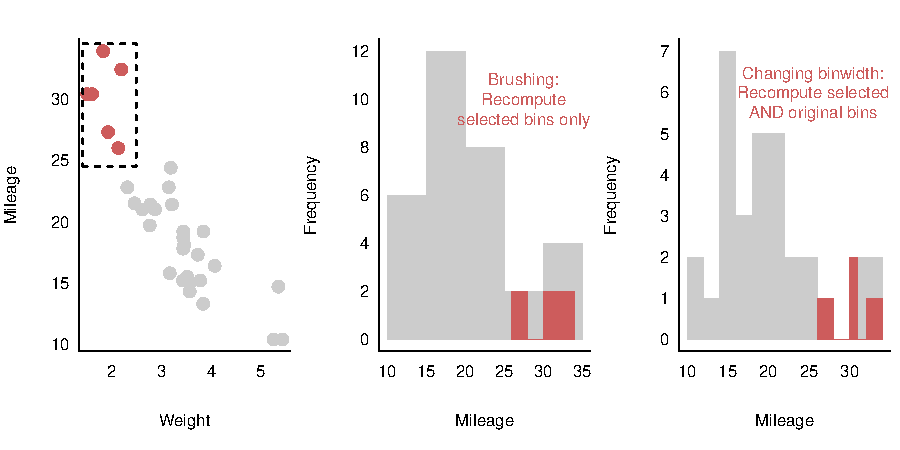
\includegraphics[height=70mm]{./figure03.pdf}
\caption{Reactive computations cascade}
\label{fig:reactivecascade}
\end{figure}

Importantly, these reactive computations can cascade and form hierarchies. Using the example of the interactive histogram above, if the histogram also responds to linked brushing, we have reactivity occuring on two different levels, as shown in Figure \ref{fig:reactivecascade}. Firstly, when linked brushing occurs, we only need to recompute the number of cases within each bin belonging to the selection. However, if the width of the bins changes, we need to recompute both the number of cases within each bin belonging to the selection as well as the number of cases within the original, unselected bins.    

\subsubsection{Visual and Computational Coherency}
\label{sec:coherency}

Perhaps more importantly, different types of interaction also place a limit on what summaries will be computationally and visually coherent. For example, suppose we have an interactive visualization that consists of a linked barplot and a scatterplot. Further, let's suppose that the barplot displays the means of some continuous variable, within the levels of the variable on the x-axis (this type of plot is also sometimes called "dynamite plot", when error bars are shown). We want the user to be able to perform linked brushing on the two plots in a reciprocal way - clicking-and-dragging to select points in the scatterplot should highlight parts of the corresponding bar or bars, and vice versa, selecting a bar should highglight the corresponding points.

We immediately run into several problems. The first is shown in Figure \ref{fig:empty}: how do we draw an empty selection? In a barplot of sums or counts, 0 is a meaningful default value, since the sum or count of a set with no elements is zero. However, the mean of an empty set is not defined. We could simply not draw the bar, but this will decohere the statistical summary from the visual representation: the absence of a bar may signal that either no cases are selected and the mean is undefined, or that there are selected cases and their mean is equal to the lower y-axis limit.

\begin{figure}[H]
\centering
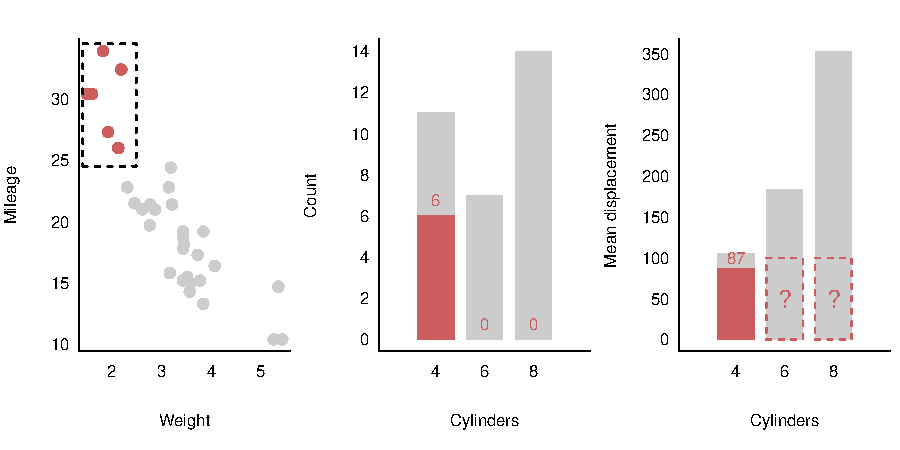
\includegraphics[height=70mm]{./figure01.pdf}
\caption{Sum/count of empty selection is zero but the mean of an empty selection is undefined}
\label{fig:empty}
\end{figure}

Second, if there are multiple selections present within a single x-axis variable level, how do we draw them? In a sum or count bar, we can stack selected groups on top of each other, and the total height of the stacked bar is equal to the sum of the heights of the sub-bars. This is not the case for mean. The mean of the group means does not have to equal the grand mean, and there is no idiosyncratic way of visually combining multiple means together. We could draw the means side-by-side as separate bars (a technique called "dodging" in \texttt{ggplot2}), however, this complicates the two-way reciprocal nature of the linked brushing - the user can no longer simply select the single unambiguous stacked bar, but instead has to learn by experience whether they can select one of the dodged group bars individually or whether they have to select all bars jointly, or some combination of both.

\begin{figure}[H]
\centering
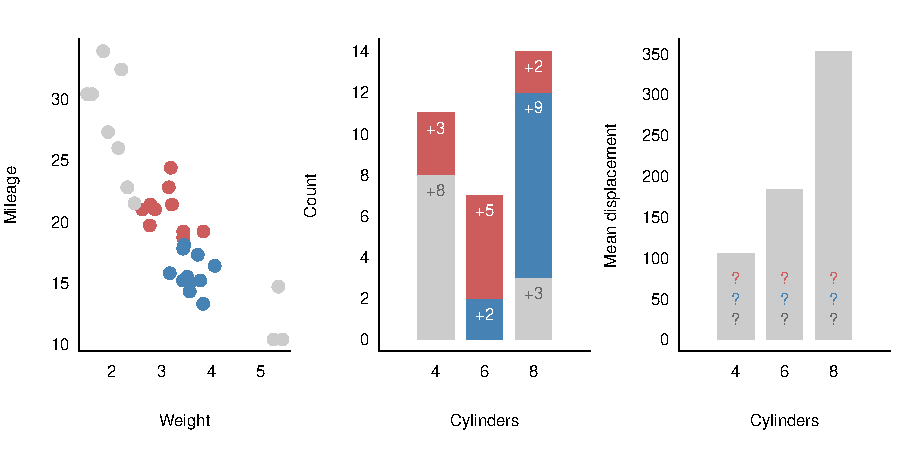
\includegraphics[height=70mm]{./figure02.pdf}
\caption{Sums/counts can be stacked but means cannot}
\label{fig:empty}
\end{figure}

Finally, and thirdly, when computing the mean, we have to keep track of two quantities: running sum and running count. If we wanted to combine two means, we would need to have access to both, not just the computed values. In contrast, for sum and count we need to keep track of one value only and the values can be combined without reference to anything else. This is not a big problem with mean and the computation can still be easily parallelized, but other types of summaries may be more tricky.

\subsubsection{Need for Structure}

The picture that emerges is that, when it comes to interactive data visualization, some types of statistical summaries are better than others. Specifically, when more complex types of interactions are desired, such as reciprocal two-way linked brushing, not every kind of statistical summary will do. It is important to map out what types of constraints should statistical summaries meet in order to "work" and lead to visually and computationally coherent visualizations. Only by imposing some kind of structure can we lay the foundations for a true mid-level interactive data visualization system. 


\subsection{Few Relevant Bits of (Applied) Category Theory}

Category theory is a branch of mathematics concerned with the study of universal structures and relations. It was developed as a way of unifying historically distinct areas of math such as abstract algebra, topology, and linear algebra. At the present time, it is also gaining traction in more applied fields, especially computer science and functional programming. Even a very basic complete treatment would be far outside the scope of the present proposal, however, few relevant pieces will be presented in a greatly simplified way, introducing examples from programming when relevant. The treatment here follows mainly from \cite{fong2019} and \cite{Milewski2018}, as well as \cite{leinster2014}.

\subsubsection{Functions}
\label{sec:functions}

Functions are the most fundamental building block of category theory (as well as many other areas of mathematics). In their more general form, they are also known as "morphisms" or "mappings". A function can be described in the following way: given two sets, the set of sources $S$ and the set of targets $T$, a function is a subset $F \subseteq S \times T$ containing all source-target pairs $(s, t)$, such that for all $s \in S$ there exists a unique a $t \in T$. The sets $S$ and $T$ are also known as the domain and codomain, respectively. In programming terms, we should be hypothetically able to implement any function as a lookup table (in practice, this is only feasible when the number of possible arguments is finite and small - but then it can be handy a technique, called \textit{memoization}).  

A function which covers all of its codomain, i.e. one for which, for all $t \in T$, there exists an $s \in S$ such that $f(s) = t$ is called \textit{surjective} or \textit{onto}. A function which has a unique element in the codomain for every element in the domain, i.e. one for which for all $s_1, s_2 \in S$ and $t \in T$, if $f(s_1) = t$ and $f(s_2) = t$, $s_1 = s_2$, is called \textit{injective} or \textit{one-to-one}. Also, for any given subset $T_i \subseteq T$, we can define \textit{pre-image} as the subset of $S$ that maps into $T_i$: $f^{-1}(T_i) = \{ s \in S : f(s) \in T_i \}$. Finally, functions can be composed: if we have two functions $f: X \to Y$ and $g: Y \to Z$, we can combine them into a new function $h = g \circ f$ such that $h: X \to Z$, i.e. $h(x) = g(f(x))$. 

\subsubsection{Partitions}

We can do many things with functions, and one fundamental operation we can do with them is to form \textit{partitions}. Specifically, given a set $A$ and a set of part labels $P$, we can use a surjective function $f: A \to P$ to assign every element in $A$ a part label in $P$. Further, if we then take one of the part labels $p \in P$ and pull it back through $f$ to its pre-image $f^{-1}(p) \subseteq A$, we will then recover the corresponding part $A_p \subseteq A$. We can use this to define partitions in another way, without reference to $f$: a partition of $A$ consists of a set of part labels $P$, such that, for all $p \in P$, there is a non-empty subset $A_p \subseteq A$ and:

$$A = \bigcup_{p \in P} A_p \qquad \text{and} \qquad \text{if } p \neq q, A_p \cap A_q = \varnothing \qquad (\forall p, q \in P)$$

I.e. the parts jointly cover the entirety of $A$ and there is no overlap between their elements. Further, if we have two sets of part labels $P$ and $P'$, and if for every $p \in P$ there exists a $p' \in P'$ such that $A_p = A_{p'}$, the partitions are in some way fundamentally the same. The labels $p \in P$ and $p' \in P'$ may be superficially different, but the two structures encode the same information. This phenomenon is known as \textit{isomorphism}, and will be expounded on in more detail in Section \ref{sec:categories}.  

\subsubsection{Preorders}

Another class of fundamental structures in category theory are preordered sets or \textit{preorders}. A preorder consists of a set $X$ and a binary relation on $X$, often denoted $\leq$, such that:

\begin{enumerate}
\item $x \leq x$ (reflexivity)
\item if $x \leq y$ and $y \leq z$ then $x \leq z$ (transitivity)
\end{enumerate}

Further, if we have one additional property:

\begin{enumerate}
\setcounter{enumi}{2}
\item If $x \leq y$ and $y \leq x$, then $x = y$ (anti-symmetry)
\end{enumerate}

Then we can speak of a partially ordered set, or \textit{poset}. Finally, with one more property:

\begin{enumerate}
\setcounter{enumi}{3}
\item Either $x \leq y$ or $y \leq x$ (comparability)
\end{enumerate}

We can speak of a \textit{total order}. Examples of total orders (which are also by definition posets and preorders) include the set of natural numbers $\mathbb{N}$, reals $\mathbb{R}$, booleans $\mathbb{B} = \{ \text{True, False} \}$, etc... An example of a poset which is not a total order is a phylogenetic tree: a species \textit{Homo sapiens} can be thought of as being in a subordinate relationship ($\leq$) to the genus \textit{Homo} and the great ape family, but in no comparable relationship to the species \textit{Canis familiaris}.

\subsubsection{Monoids}

\textit{Monoids} are a simple yet surprisingly useful structure in category theory. Specifically, a monoid is a tuple $(M, e, \otimes)$ consisting of:

\begin{enumerate}
\item An object (set) $M$
\item A "neutral" or "empty" element $e \in M$ called the \textit{monoidal unit}
\item A binary function $\otimes: M \times M \to M$ called the \textit{monoidal product}
\end{enumerate}

Such that, for all $m, m_1, m_2, m_3 \in M$: 

\begin{enumerate}
\renewcommand{\theenumi}{\alph{enumi}}
\item $e \otimes m = m \otimes e = m$ (unitality)
\item $(m_1 \otimes m_2) \otimes m_3 = m_1 \otimes (m_2 \otimes m_3) = m_1 \otimes m_2 \otimes m_3$ (associativity)
\end{enumerate}

In plain English, monoids encapsulate the idea that \textit{the whole is exactly the sum of its parts} (where "sum" can be any arbitrary function that fulfills the properties). Examples of monoids include addition of natural numbers $(\mathbb{N}, 0, +)$, multiplication of reals $(\mathbb{R}, 1, *)$, and matrix multiplication $(\mathbf{Matrix}, \mathbf{I}, \cdot)$, where $\mathbf{I}$ is the identity matrix and the $\cdot$ infix operator is typically omitted by convention. As counterexample, exponentiation is not a monoid, because because it is not associative ($x^{(y^z)} \neq (x^y)^z$). 

Another important aside is that the set $M$ does not need to involve any numerical quantities. For example, given any set $S$, the set union $(S, \varnothing, \cup)$ and set intersection $(S, S, \cap)$ are also monoids. String concatenation (e.g. the \texttt{paste()} function in R) is also a perfectly valid monoid: 

\begin{itemize}
\item \texttt{paste("hello", "") == paste("", "hello") == "hello"}
\item \texttt{paste("hello", paste("world", "bye")) == paste(paste("hello", "world"), "bye")}
\end{itemize}

Monoids can be further specialized by imposing additional properties. For example, with:

\begin{enumerate}
\renewcommand{\theenumi}{\alph{enumi}}
\setcounter{enumi}{2}
\item $x \otimes y = y \otimes x$ (commutativity/symmetry)
\end{enumerate}

We can make it so that the direction of applying the monoidal product does not matter (which would still admit regular addition, multiplication, set union, and set intersection, but not matrix multiplication and string concatenation). Additionally, if $M$ is a preorder, we can impose an additional constraint:

\begin{enumerate}
\renewcommand{\theenumi}{\alph{enumi}}
\setcounter{enumi}{3}
\item If $x_1 \leq x_2$ and $y_1 \leq y_2$, $x_1 \otimes y_1 \leq x_2 \otimes y_2$ (monotonicity)
\end{enumerate}

If all four properties a), b), c), and d) hold, we speak of a \textit{symmetric monoidal preorder}. 

In programming, monoids are most typically encountered in the context of arrays, whereby the elements of an array can be iteratively absorbed into a single value, through functions/methods called conventionally \texttt{reduce}, \texttt{fold}, or \texttt{accumulate}. Examples include the \texttt{Reduce()} function in R, \texttt{Array.reduce()} method in JavaScript, \texttt{fold} function in Haskell. Importantly, while \texttt{reduce/fold} are most often used with arrays, their generic forms are polymorphic and can be applied to arbitrary datastructures that implement the interface e.g. trees \citep{braithwaite2019}. One handy, "free" fact about monoidal operations is that they can be readily parallelized - since the end-result of applying the operation recursively to parts is the same as applying it once to the whole, we are free to split the data across multiple clusters or machines.  

\subsubsection{Categories}
\label{sec:categories}

A monoid is actually a special case of a much more general concept called \textit{category}. A category $\mathcal{C}$ consists of:

\begin{enumerate}
\item A collection of elements $\text{Ob}(\mathcal{C})$ called the \textit{objects} of $\mathcal{C}$
\item For every pair of objects $a, b \in \text{Ob}(\mathcal{C})$, a set $\mathcal{C}(a, b)$ of \textit{morphisms} from $a$ to $b$ ($f \in \mathcal{C}(a, b)$ can also be denoted $f: a \to b$)
\item For every object $a$, one morphism $\text{id}_a : a \to a$ called the \textit{identity morphism}
\item For every three objects $a, b, c$ and every two morphisms $f : a \to b$ and $g : b \to c$, a \textit{composite morphism} $h : a \to c = g \circ f $ 
\end{enumerate}

Such that:

\begin{enumerate}
\renewcommand{\theenumi}{\alph{enumi}}
\item For any morphism $f: a \to b$, $f \circ id_a = f = id_b \circ f$ (unitality)
\item For any four objects $a_1, a_2, a_3, a_4 \in \text{Ob}(\mathcal{C})$ and morphisms $f: a_1 \to a_2$, $g: a_2 \to a_3$, and $h: a_3 \to a_4$, $h \circ (g \circ f) = (g \circ h) \circ f = g \circ h \circ f$ (associativity)
\end{enumerate}


As was mentioned in Section \ref{sec:functions}, morphisms can be thought of as generalizations of functions: they take one object within a category to another object within the same category, and their composition is associative, just like with regular functions. However, unlike in regular functions, the objects in the category are left unspecified and do not have form elements of any set. The identity morphism guarantees there is always at least one way to start and arrive at the same object, and its composition with other morphisms has no effect.

Returning to monoids, these can recast as a category with one object with a single non-identity morphism going from the object back to itself. As a concrete example, given the monoid $(\mathbb{N}, 0, +)$, we can represent this as a category with a single object $z$ and a morphism $f$ (and identity morphism $id_a$). The identity morphism will then play the role of the monoidal unit $e = id_a$, function composition will play the role of the monoidal product, and the number of times we compose the function will determine the element of the set: $\{0, 1, 2, \ldots \} = \{id_a, f, (f \circ f), (f \circ f \circ f), \ldots \}$. The associativity and unitality properties of monoids will be fulfilled as a result of the same properties being defined on categories.  


% ----------------------------------------------------------------------
\section{So What's New?}
\label{sec:whatsnew}

As was laid out in the previous sections, when compared to traditional, static visualization, interactive data visualization presents an idiosyncratic set of challenges and considerations. Specifically, when drawing and interacting with statistical summaries of the data, the user needs to carefully navigate the landscape of these summaries, with only some producing visually and computationally coherent results. The goal of this project is to map out this landscape, and develop theory that will allow everyone to produce coherent interactive graphics. To this end, ideas and concepts from category theory will be used. As a first taste, returning to the problem of two-way linked brushing described in \ref{sec:coherency}, through the lense of category theory it is clear that the summaries that will produce coherent graphics need to fulfill the contract of a monoid, or more specifically \textit{symmetric monoidal structure on total order} (since the things we draw such as length, width, area are all in $\mathbb{R}^+$, and the direction of combining the selections should not matter)      

Further, the project also seeks to apply this theory and implement an interactive data visualization system which adheres to it. To this end, a prototype has already been developed in JavaScript and is available at: \texttt{https://github.com/bartonicek/plotscaper}. Going forward, the following broad goals will be pursued (see Section \ref{sec:goals} for a detailed breakdown):  

\begin{enumerate}

\item Map out the boundaries and constraints of statistical summaries as they relate to interactive data visualization systems 
\item Develop theory for an implementation of a mid-level system
\item Implement the system
\item Communicate the findings

\end{enumerate}


% ----------------------------------------------------------------------
\section{Data and Special Needs}
\label{sec:data}

The use of the system will be tested out on datasets available in the public domain such as the \texttt{diamonds} dataset in R. For these data sets, no ethics or disclosure statements are necessary. Possible collaboration with working scientists and corresponding data access may be negotiated at a later date.  

The student's own personal computer should be sufficient to produce the developing and testing the system. Should extra computing resources become necessary, the student should be able to inquire and be granted access to the \textbf{Ihaka server} (\texttt{ihaka.stat.auckland.ac.nz.}) using SSH connection. Other options such as the New Zealand eScience Infrastructure (\textbf{NeSI}) should be available too. 

The packages produced as part of the project will be published for free as open-source software, under the MIT license \citep{mit2023}. No additional ethics approvals are necessary. 

% ----------------------------------------------------------------------
\section{Budget}

Development of open-source software is not very budget-intensive. The work related to the project will be funded by the University of Auckland Doctoral Scholarship. Expenses related to conferences (registration fees, travel) may be funded via the Postgraduate Research Student Support (PReSS) account, with an annual allocation of \$1200 NZD. 

% ----------------------------------------------------------------------
\section{Objectives and Goals}
\label{sec:goals}


The objective(s) of this research project are to:

\begin{enumerate}

\item
Map out boundaries and constraints that statistical summaries in a mid-level interactive data visualization system should meet
  \begin{enumerate}
  \item Describe what contracts do graphical primitives and underlying statistical summaries need to uphold in order to be interactable with in a coherent and predictable way
  \item Use concepts from category theory to describe the necessary structures
  \item Consider links to functional programming  
  \end{enumerate}

\item Implement the system in JavaScript (provisionally named \texttt{plotscape})
  \begin{enumerate}
  \item Use mainly plain ES2020, possibly incorporate basic utility libraries such as a reactive programming library and functional programming library
  \item Use the HTML \texttt{canvas} element as a drawing utility, explore using WebGL and other frameworks for performance
  \item Profile and test relevant parts of the code
  \item Publish as an \texttt{npm} package
  \item Provide a full documentation for any functions, classes, etc...
  \end{enumerate}

\item Implement a high-level interface to the system in R (provisionally named \texttt{plotscaper})
  \begin{enumerate}
  \item Provide a full documentation for all functions
  \item Provide a package vignette
  \item Pass all \texttt{CRAN} checks and publish on \texttt{CRAN} 
  \end{enumerate}
  
\item Publish an article in a peer-reviewed academic journal such as the \textit{Journal of Statistical Software}

\item Present finding at conferences and user groups such as \textbf{useR!} and \textbf{IEEE VIS}

\end{enumerate}

% ----------------------------------------------------------------------
\section{Deliverables and Program Schedule}
\label{sec:timeline}




\begin{table}[hh]
\caption{
Timeline for my thesis.
Itemize the list of deliverables with specific dates so that
you can make concerted effort to achieve them.
Here are \textit{some} activities---fill in more.
}
\centering
\ ~~~~ \\
\label{tab:timeline}
\begin{tabular}{|c|l|}
\hline
Date & Activity \\
\hline
2022-03-01 & Enrolled in Research Master's in Statistics, backdated provisional PhD registration. \\
2022-11-07 & Made a Github commit of the initial fully working prototype of \texttt{plotscaper}. \\
2022-11-22 & Gave talk at the NZSA Unconference, received Outstanding Student Presentation award. \\
2023-02-13 & Completed DELNA. \\
2023-03-10 & Attended central doctoral induction. \\
2023-04-07 & Presented my research at Iowa State University Graphics Group \\
2023-04-13 & Attended FoS doctoral induction. \\
2023-05-14 & Present my research at a PYR seminar \\
2023-08-01 & Finalize version 1.0 of \texttt{plotscape} and publish on \texttt{npm} \\
2023-09-01 & Attend a statistical computing/data visualization conference \\
2023-12-01 & Submit my first paper to \textit{Journal of Statistical Software} (co-authored with supervisors). \\
2024-01-01 & Finalize version 1.0 of \texttt{plotscaper} and publish on \texttt{CRAN}. \\
2024-03-01 & Begin work on formalizing the manuscript \\
2024-06-01 & Attend a statistical computing/data visualization conference \\
2025-03-01 & Submit my PhD thesis. \\
\hline
\end{tabular}
\end{table}



I have fulfulled all my first year requirements. These are:

\begin{enumerate}

\item \textit{Attend the Central Doctoral Induction}: 2023-03-10
\item \textit{Attend the FoS Doctoral Induction}: 2023-04-13
\item \textit{Complete DELNA screening}: 2023-02-13
\item \textit{Complete a health and safety risk assessment (if required)}: not required
\item \textit{Gain ethics approval (if required)}: not required
\item \textit{Complete training and development needs analysis}: completed prior to transferral from Research Master's
\item \textit{Gain approval for your full thesis proposal}: in process
\item \textit{Give an oral presentation of your work}: PYR seminar being scheduled for May
\item \textit{Produce a substantial piece of written work}: roughly 80~percent Research Master's thesis submitted to primary supervisor for review, 
code repositories available for review on Github at \texttt{https://github.com/bartonicek}
\item \textit{Discuss your research with your Confirmation Review Committee}: in process \newline \newline

Additional first year milestones:

\item \textit{Attend 10 departmental seminars}: Currently 8 attended, I have had only about 3 months to attend departmental seminars (I did not know about this requirement before I decided to transfer from Research Master's) but have tried to attend as many as possible.
\item \textit{Engage with other scholars}: Presented research at the NZSA Uncoference 2022 (and received an award) as well as at Iowa State University Graphics Group
\item \textit{Review existing methods and literature on approaches to interactive statistical graphics}: Completed as part of the submitted draft of Research Master's Thesis
\item \textit{Implement a software prototype capable of producing linked interactive plots with support for different types of brushing}: implemented in \texttt{plotscape}


\end{enumerate}


\begin{table}[H]
\caption{
\textbf{Seminars I have attended}.
First section includes departmental seminars.
Second section includes seminars from another UoA department.
Third row includes conference talks.
Fourth row includes talks I presented (these do not count towards seminar attendance as far as I am aware but I thought it may still be useful to include them) \newline
\textbf{Note}:
I filled in the required document and submitted it within the required time period after each seminar I attended.
}
\centering
\ ~~~~ \\
\label{tab:seminars}
\begin{tabular}{|c|l|p{10cm}|}
\hline
Date & Speaker & Title \\
\hline
2023-01-27 & Bradley Drayton &
A Talk About Simulations \\
%
2023-02-10 & Rob Gould &
K-12 Data Science or Statistics? Is a Distinction Needed? \\
%
2023-02-22 & Maartje van de Vrugt &
Experiences of an OR Specialist Advising in a Hospital: Reducing Cancellations and
Scheduling Re-work at Outpatient Departments of Amsterdam UMC \\
%
2023-03-07 & Chaitanya Joshi &
Eliciting Informative Priors using Expert decision-making \\
%
2023-03-07 & Fabrizio Ruggeri &
Fast and Likelihood-Free Parameter Estimation for Dynamic Queueing Networks: The
Case of the Immigration Queue at an International Airport \textit{(counts as 1/2 seminar)} \\
%
2023-03-07 & Petra Tang &
A Parametric Approach to estimate Spectral Density of Gravitational Wave Signal from
BPASS Galactic White Dwarf Binary Population \textit{(counts as 1/2 seminar)} \\
%
2023-03-30 & Matt Edwards &
The Good, the Bad, and the Ugly of Working at StatsNZ \\
\hline

2023-04-12 & Christopher Horvat &
How Do the Floes Flow? Discrete-Element Modelling of Sea Ice-Ocean Dynamic Coupling in the Marginal Ice Zone. \newline Department of Physics. \\

\hline

2022-11-23 & Tilman Davies & Nearest-Neighbour Gaussian Processes. \newline NZSA Unconference 2022. \\

\hline
%
2022-11-22 & Adam Bartonicek (presented) & Interactive Data Exploration with \texttt{plotscaper}. \newline NZSA Unconference 2022 \\
%
2023-04-07 & Adam Bartonicek (presented) & \textit{Same title as above}. \newline Iowa State University Graphics Group \\

\hline

\end{tabular}
\end{table}








% ----------------------------------------------------------------------
\section*{Appendix~A}

\addcontentsline{toc}{section}{References}
\bibliographystyle{./elsart-harv} % elsart-harv,plain,unsrt,alpha
\bibliography{./references}



\end{document}


